\documentclass[a4paper,12pt]{article}

\usepackage[utf8]{inputenc}
\usepackage[left=0.5in,right=0.5in,top=1in,bottom=1in]{geometry}
\usepackage{amsmath,amssymb,amsfonts}
\usepackage{pgfplots,graphicx,calc,changepage,caption}
\pgfplotsset{compat=newest}
\usepackage{enumitem}
\usepackage{fancyhdr}
\usepackage[colorlinks = true, linkcolor = black]{hyperref}

% Syntax highlighting
\usepackage{listings}
\usepackage{xcolor}

\definecolor{codegreen}{rgb}{0.40,0.62,0.07}
\definecolor{codegray}{rgb}{0.5,0.5,0.5}
\definecolor{codeblue}{rgb}{0.09,0.57,0.73}
\definecolor{backcolour}{rgb}{1,1,1}

\lstdefinestyle{mystyle}{
    backgroundcolor=\color{backcolour},   
    commentstyle=\color{codegreen},
    keywordstyle=\color{magenta},
    numberstyle=\tiny\color{codegray},
    stringstyle=\color{codeblue},
    basicstyle=\ttfamily\small,
    breaklines=true,                     
    keepspaces=true,                 
    numbers=left,                    
    numbersep=5pt,                  
    showspaces=false,
    showstringspaces=false,
    showtabs=false,                  
    tabsize=4
}

\lstset{style=mystyle}

\newcommand{\nats}{\mathbb{N}}
\newcommand{\reals}{\mathbb{R}}
\newcommand{\rats}{\mathbb{Q}}
\newcommand{\ints}{\mathbb{Z}}
\newcommand{\comps}{\mathbb{C}}
\newcommand{\pols}{\mathcal{P}}
\newcommand{\cants}{\Delta\!\!\!\!\Delta}
\newcommand{\eps}{\varepsilon}
\newcommand{\st}{\backepsilon}
\newcommand{\abs}[1]{\left| #1 \right|}
\newcommand{\dom}[1]{\mathrm{dom}\left(#1\right)}
\newcommand{\for}{\text{ for }}
\newcommand{\dd}[1]{\mathrm{d}#1}
\newcommand{\spn}{\mathrm{sp}}
\newcommand{\nul}{\mathcal{N}}
\newcommand{\col}{\mathrm{col}}
\newcommand{\rank}{\mathrm{rank}}
\newcommand{\norm}[1]{\lVert #1 \rVert}
\newcommand{\inner}[1]{\left\langle #1 \right\rangle}
\newcommand{\pmat}[1]{\begin{pmatrix} #1 \end{pmatrix}}
\renewcommand{\and}{\text{ and }}

\newsavebox{\qed}
\newenvironment{proof}[2][$\square$]
    {\setlength{\parskip}{0pt}\par\textit{Proof:} #2\setlength{\parskip}{0.25cm}
        \savebox{\qed}{#1}
        \begin{adjustwidth}{\widthof{Proof:}}{}
    }
    {
        \hfill\usebox{\qed}\end{adjustwidth}
    }

\pagestyle{fancy}
\fancyhead{}
\lhead{Caleb Jacobs}
\chead{APPM 5600: Numerical Analysis I}
\rhead{Homework \#6}
\cfoot{}
\setlength{\headheight}{35pt}
\setlength{\parskip}{0.25cm}
\setlength{\parindent}{0pt}

\begin{document}
\section*{Problems}
\begin{enumerate}[label = \arabic*)]
	\item In class, we showed that
	\begin{equation}
		p_{k+1} = r_{k+1}- \frac{\inner{p_k,r_{k+1}}_A}{\norm{p_k}_A^2}p_k. \label{equ:1}
	\end{equation}
	\begin{enumerate}[label = (\alph*)]
		\item Using the fact that $ r_{k+1} = r_k - \alpha_k A p_k $ and $ r_{k+1}^T r_k = 0 $, show that $ \inner{p_k, r_{k+1}}_A = -\frac{\norm{r_{k+1}}_2^2}{\alpha_k} $.
		
		\begin{align*}
			0 = r_{k+1}^T r_k &= r_{k+1}^T (r_{k+1} + \alpha_k A p_k) \\
			&= r_{k+1}^T r_{k+1} + \alpha_k r_{k+1} A p_k \\
			\implies r_{k+1} A p_k &= -\frac{r_{k+1}^T r_{k+1}}{\alpha_k}
		\end{align*}
		which implies
		\[
			\inner{p_k, r_{k+1}}_A = -\frac{\norm{r_{k+1}}_2^2}{\alpha_k}.
		\]
		
		\item Rewrite $ \norm{p_k}_A^2 $ in terms of $ r_k $ and $ \alpha_k $.
		
		\begin{align*}
			\norm{p_k}_A^2 &= p_k^T A p_k \\
			&= \left(r_k - \frac{\inner{p_{k-1}, r_k}}{\norm{p_{k-1}}_A^2} p_{k-1} \right)^T \frac{1}{\alpha_k}(r_k - r_{k+1}) \\
			&= \frac{1}{\alpha_k}(r_k^T r_k - r_k^Tr_{k+1}) \quad \text{because $ p_{k-1} $ is orthogonal to $ r_k $ and $ r_{k+1} $} \\
			&= \frac{1}{\alpha_k}r_k^T r_k \\
			&= \frac{1}{\alpha_k} \norm{r_k}_2^2.
		\end{align*}
		
		\item Plug these expressions into \eqref{equ:1} to get a technique for evaluating the next basis vector for the residual space without any applications of the matrix $ A $.
		\begin{align*}
			p_{k+1} &= r_{k+1} - \left(-\frac{\norm{r_{k+1}}_2^2}{\alpha_k}\right)\left(\frac{\alpha_k}{\norm{r_k}_2^2}\right) p_k \\
			&= r_{k+1} + \left(\frac{\norm{r_{k+1}}_2}{\norm{r_k}_2}\right)^2 p_k.
		\end{align*}
	\end{enumerate}

	\newpage
	\item Consider a sparse $ 500 \times 500 $ matrix $ A $ constructed as follows.
	\begin{itemize}[topsep = 0pt]
		\item Put a $ 1 $ in each diagonal entry.
		\item In each off-diagonal entry put a random number from the uniform distribution on $ [-1,1] $ but make sure to maintain symmetry. Then replace each off-diagonal entry with $ \abs{A_{ij}} > \tau $ by $ 0 $, where $ \tau $ for $ \tau = 0.01, 0.05, 0.1, $ and $ 0.2 $.
	
	\end{itemize}
		
	Take the right hand side to be a random vector $ b $ and set the tolerance to $ 10^{-10} $.
	
	\begin{figure}[h!]
		\centering
		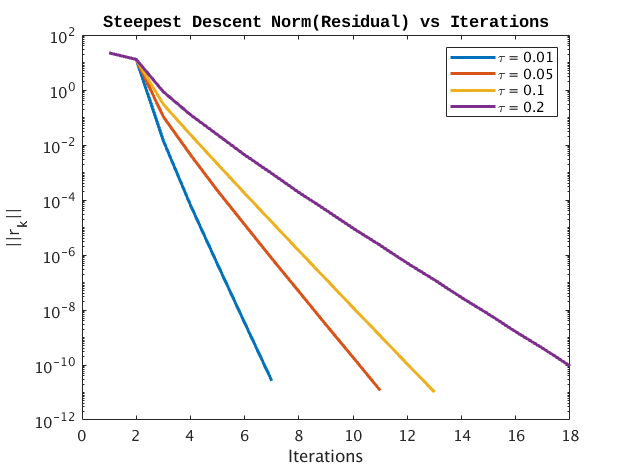
\includegraphics[width = 0.45\textwidth]{images/steepestdescent.png}
		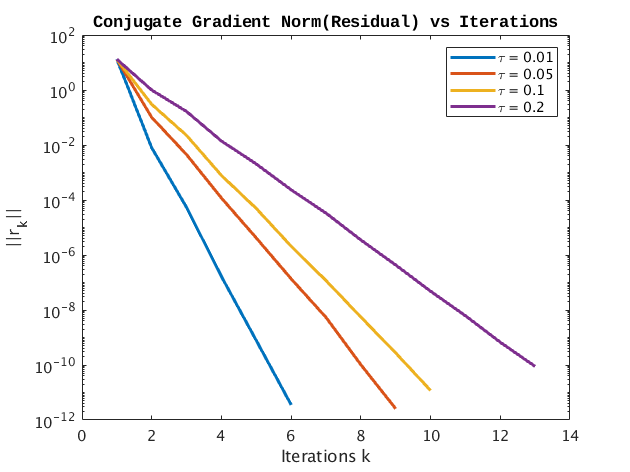
\includegraphics[width = 0.45\textwidth]{images/conjgrad.png}
		\captionsetup{width=0.8\textwidth}
		\caption{Convergence plot of the steepest descent method (left) and the conjugate gradient method (right).}
		\label{fig:conv}
	\end{figure}
	
	\begin{enumerate}[label = (\alph*)]
		\item Write the Steepest Descent (SD) and Conjugate Gradient (CG) solver.
		
		\begin{center}
			\emph{My code is given at the end of the document.}
		\end{center}
		
		\item Apply SD to solve each of the linear systems and plot the residual for each iteration $ \norm{r_n} $ versus the iteration $ n $ on a \emph{semilogy} scale. 
		
		Using SD from my code, the convergence plot can be seen in left graphic of Figure \ref{fig:conv}.
		
		\item Apply CG to solve each of the linear systems and plot the residual for each iteration $ \norm{r_n} $ versus the iteration $ n $ on a \emph{semilogy} scale.
		
		Using CG from my code, the convergence plot can be seen in right graphic of Figure \ref{fig:conv}.
		
		\item What do you observe about the convergence of these methods? If the methods do not converge for any choices of $ \tau $ explain what's happening.
		
		In the case of my stochastic matrix, both methods converged for each value of $ \tau $ but with a few key differences. The most prominent difference is that SD routinely took a few iterations longer to converge than CG for each $ \tau $. Furthermore, the very first iteration of SD did see much improvement in the residual while CG usually had it's greatest reduction in the residual for the very first iteration. We can explain the greatest initial improvement of CG by noting that CG resolves the solution in the direction of the eigenvectors which the greatest modulus eigenvalues. Thus, when we apply CG to each matrix, CG resolves the eigenvalues with magnitude one because they are the most prominent in each matrix. Therefore, the first iteration of CG makes the most ground in solving the system.
		
		Another trend to note that is true for both SD and CG plots is the decrease in convergence rate as $ \tau $ increases. As $ \tau $ increases, the eigenvalues of each matrix become more spread out and the matrix might even obtain some negative eigenvalues which means the matrix is no longer SPD. Thus, as $ \tau $ increases the conditioning of each system increases causing each method to converge at a slower rate.
		
		\item How do the residual compare with the error bounds provided in class?
		
		For SD, the error bound from class states that
		\[
			\norm{e_{k+1}}_A \leq \sqrt{\frac{\lambda_{max} - \lambda_{min}}{\lambda_{max} + \lambda_{min}}} \norm{e_k}_A.
		\]
		For my random matrices, we have
		\[
			\sqrt{\frac{\lambda_{max} - \lambda_{min}}{\lambda_{max} + \lambda_{min}}} = \begin{cases}
				9.360477432564406e-02, & \tau = 0.01 \\
				2.583812920609023e-01, & \tau = 0.05 \\
				3.154992405543542e-01, & \tau = 0.1   \\
				4.939322020464611e-01, & \tau = 0.2
			\end{cases}.
		\]
		Thus, looking at our initial guess of $ 0 $ which has an approximate error of $ 10^1 $ and $ \tau = 0.01 $, we would expect SD to converge with a tolerance of $ 10^{10} $ in under 10 iterations because our error coefficient is on the order of $ 10^{-2} $. This is exactly what our residual plot shows and each iteration appears to increase the accuracy by 2 digits! For each of the other values of $ \tau $, we should expect convergence in a little over 10 iterations because the error coefficient is on the order of $ 10^{-1} $ which means the we should get about another digit of accuracy per iteration. Once again, our residual plot for SD shows this trend as well.
		
		For CG, our error bound from class states
		\[
			\norm{e_{k}}_A \leq 2 \left(\frac{\sqrt{\kappa(A)} - 1}{\sqrt{\kappa(A)} + 1}\right)^k \norm{e_0}_A.
		\]
		For my random matrices, we have
		\[
			\frac{\sqrt{\kappa(A)} - 1}{\sqrt{\kappa(A)} + 1} = \begin{cases}
				4.381010972533616e-03, & \tau = 0.01 \\
				3.341772346442987e-02, & \tau = 0.05 \\
				4.989378202454497e-02, & \tau = 0.1 \\
				1.238557836168690e-01, & \tau = 0.2
			\end{cases}.
		\]
		Using these error coefficients for the first three values of $ \tau $, we would expect CG to converge in under 10 iterations because the error which starts at about $ 10^1 $ decreases by $ 10^{-3} $ or $ 10^{-2} $ at each iteration. This is exactly what our plot for the convergence of CG shows. Finally, for $ \tau = 0.2 $, the error bound decreases by $ 10^{-1} $ at each iteration and so we should expect convergence in over 10 iterations. Once again, the convergence plot for CG shows this trend as well. 
		
		Therefore, our theoretical error bounds apply to both of our actual test problems!
	\end{enumerate}

	\item Suppose CG is applied to a symmetric positive definite matrix $ A $ with the result $ \norm{e_0}_A = 1 $, and $ \norm{e_{10}}_A = 2 \cdot 2^{-10} $, where $ \norm{e_k}_A = \norm{x_k - x^*}_A $ and $ x^* $ is the true solution. Based solely on this data,
	\begin{enumerate}[label = (\alph*)]
		\item What bound can you give on $ \kappa(A) $?
		
		To compute a bound for $ \kappa(A) $, note that the error bound for CG applied to SPD matrices is given by
		\[
			\norm{e_k}_A \leq 2 \left(\frac{1 - \sqrt{\frac{1}{\kappa(A)}}}{1 + \sqrt{\frac{1}{\kappa(A)}}}\right)^n \norm{e_0}_A = 2 \left(\frac{\sqrt{\kappa(A)} - 1}{\sqrt{\kappa(A)} + 1}\right)^n \norm{e_0}_A.
		\]
		Then, putting our given errors together, we have
		\[
			\norm{e_{10}}_A = 2 \cdot 2^{-10} \leq 2 \left(\frac{\sqrt{\kappa(A)} - 1}{\sqrt{\kappa(A)} + 1}\right)^{10} 1
		\]
		which implies
		\begin{align*}
			&&2^{-10} &\leq \left(\frac{\sqrt{\kappa(A)} - 1}{\sqrt{\kappa(A)} + 1}\right)^{10} \\
			\implies && \frac{1}{2} &\leq \frac{\sqrt{\kappa(A)} - 1}{\sqrt{\kappa(A)} + 1} \\
			\implies && \frac{1}{2}\sqrt{\kappa(A)} + \frac{1}{2} & \leq \sqrt{\kappa(A)} - 1 \\
			\implies && \frac{3}{2} &\leq \frac{1}{2}\sqrt{\kappa(A)} \\
			\implies &&  9 &\leq \kappa(A)
		\end{align*}
	
		\item What bound can you give on $ \norm{e_{20}}_A $?
		
		If we take the lower bound on $ \kappa(A) = 9 $, then we have the error bound
		\[
			\norm{e_{20}}_A \leq 2 \left(\frac{\sqrt{\kappa(A)} - 1}{\sqrt{\kappa(A)} + 1}\right)^{20} \norm{e_0}_A = 2 \cdot 2^{-20}.
		\]
	\end{enumerate}

	\item Consider the task of solving the following system of nonlinear equations.
	\[
		f_1(x,y) = 3x^2 + 4y^2 - 1 = 0 \text{ and } f_2(x,y) = y^3 - 8x^3 - 1 = 0
	\]
	for the solution $ \alpha $ near $ (x,y) = (-0.5, 0.25) $.
	\begin{enumerate}[label = (\alph*)]
		\item Apply the fixed point iteration with
		\[
			g(x) = x - \pmat{0.016 & -0.17 \\ 0.52 & -0.26} \pmat{3x^2 + 4y^2 - 1 \\ y^3 - 8x^3 - 1}.
		\]
		You can use $ (-0.5, 0.25) $ as the initial condition. How many steps are needed to get an approximation to 7 digits of accuracy?
		
		Using my code (given at the end of the document), the fixed point iteration converges in 4 iterations to an answer of 
		\[
			\pmat{x \\ y} = \pmat{-0.497251208023980 \\ 0.254078591468912}
		\]
		 which is surprisingly fast! 
		
		\item Why is this a good choice for $ g(x) $.
		
		To understand why this is a good choice for $ g(x) $, let's look at the Jacobian of $ f_1 $ and $ f_2 $ at $ (-0.5, 0.25) $:
		\[
			J = \pmat{-3 & 2 \\ -6 & 3/16}.
		\]
		Then, inverting $ J $ yields
		\[
			J^{-1} = \pmat{1/61 & -32/183 \\ 32/61 & -16/61} \approx \pmat{0.016393 & -0.174863 \\ 0.52459 & -0.262295}.
		\]
		Thus, $ J^{-1} $ is the almost exactly the same as the $ 2 \times 2 $ matrix in $ g(x) $. Furthermore, the vector function in $ g(x) $ is just the vector function formed from $ f_1 $ and $ f_2 $. All of this together implies that $ g(x) $ is sort of Newton's Method but with a fixed inverse Jacobian. Then, because our initial solution guess is close to the true solution, $ g(x) $ should almost have quadratic convergence to the solution because it is like a local Newton's method.
	\end{enumerate}
\end{enumerate}

\newpage
\section*{Code Used}
\subsection*{Problem 2}
\rule{\textwidth}{0.4pt}
	\lstinputlisting[language = matlab]{"code/Problem_2.m"}
\rule{\textwidth}{0.4pt}

\newpage
\subsection*{Problem 4}
\rule{\textwidth}{0.4pt}
	\lstinputlisting[language = matlab]{"code/Problem_4.m"}
\rule{\textwidth}{0.4pt}
\end{document}